\documentclass[12pt,letterpaper]{article}
\usepackage[latin1]{inputenc}
\usepackage{amsmath}
\usepackage{amsfonts}
\usepackage{amssymb}
\usepackage{amsthm}
\usepackage{enumerate}
\usepackage[margin=0.8in]{geometry}
\usepackage{graphicx}

\newtheorem{theorem}{Theorem}
\newtheorem{rem}[theorem]{Remark}
\newenvironment{remark}{\begin{rem}\rm}{\end{rem}}
\newtheorem{claim}[theorem]{Claim}
\newtheorem{lemma}[theorem]{Lemma}
\newtheorem{proposition}[theorem]{Proposition}
\newtheorem{corollary}[theorem]{Corollary}
\newtheorem{eg}[theorem]{Example}
\newenvironment{example}{\begin{eg}\rm}{\end{eg}}
\newtheorem{definition}[theorem]{Definition}

\newcommand{\C}{\mathbb{C}}
\newcommand{\dotp}{\boldsymbol{\cdot}}
\newcommand{\di}{\displaystyle}
\newcommand{\R}{\mathbb{R}}
\renewcommand{\S}{\mathbf{S}}
\newcommand{\x}{\mathbf{x}}
\renewcommand{\r}{\mathbf{r}}
\newcommand{\F}{\mathbf{F}}
\renewcommand{\i}{\mathbf{i}}
\renewcommand{\j}{\mathbf{j}}
\renewcommand{\k}{\mathbf{k}}
\newcommand{\abs}[1]{\lvert#1\rvert}
\newcommand{\N}{\mathbf{N}}
\DeclareMathOperator{\Real}{Re}
\DeclareMathOperator{\Img}{Im}
\newcommand{\len}[1]{\left\lVert #1\right\rVert}
\newcommand{\bbm}{\begin{bmatrix}}
\newcommand{\ebm}{\end{bmatrix}}

\author{Sean Fitzpatrick}
\title{Surface Integrals}

\begin{document}
\maketitle

This handout gives brief overview of parametric surfaces and surface integrals, with exercises.

\section{Parametric Surfaces}
Recall that a \textbf{parametric} curve in $\R^3$ can be described by a vector-valued function $\r(t) = \langle x(t), y(t), z(t)\rangle$, with $t\in [a,b]$. The tangent vector to such a curve is given by $\r'(t)=\langle x'(t), y'(t), z'(t)\rangle$. Suppose we have a level surface $S$ given by $f(x,y,z)=c$. If $C$ is a curve on $S$, and $C$ is parameterized by $\r(t)$, then $f(\r(t))=c$ for all $t\in [a,b]$. Since the curve $C$ lies along the surface $S$, it follows that any tangent vector to the curve $C$ is also tangent to the surface $S$. If $\r(t_0)=\langle x_0,y_0,z_0\rangle$, then $(x_0,y_0,z_0)\in S$, and the vector $\r'(t_0)$ lies in the tangent plane to $S$ at $(x_0, y_0, z_0)$.

\begin{figure}[h]
\begin{center}
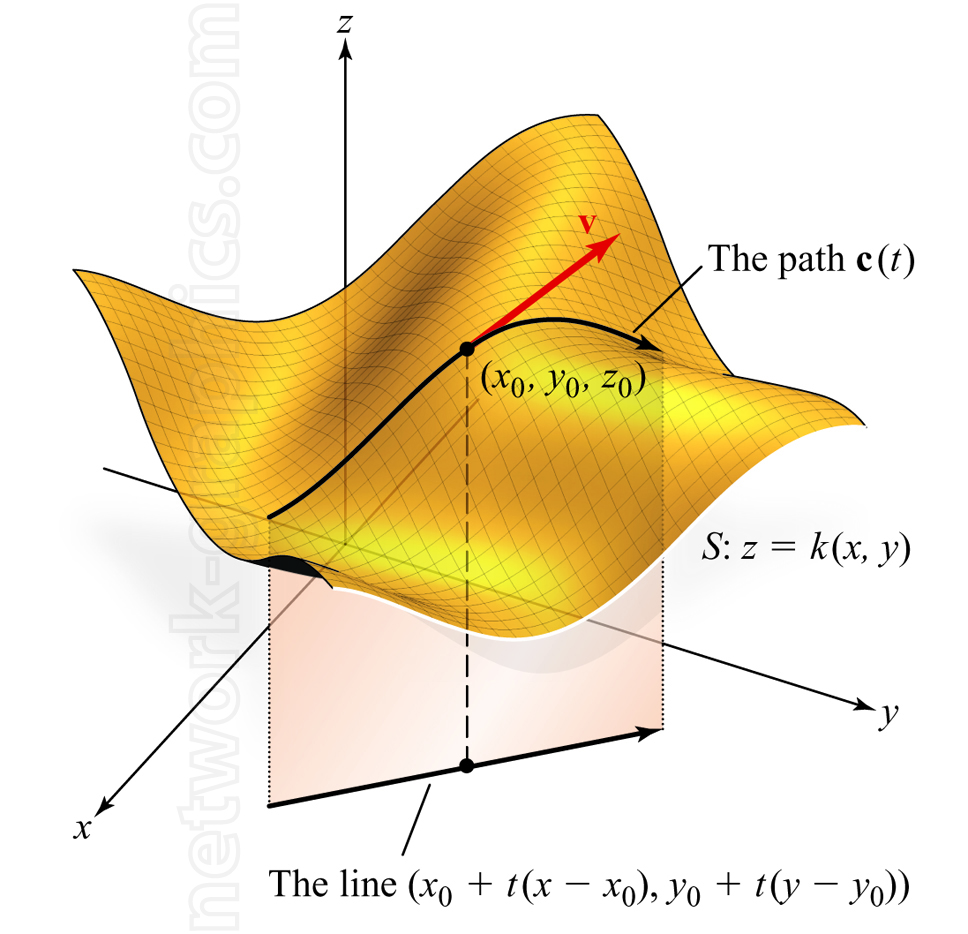
\includegraphics[width=0.5\textwidth]{curve_surf.png}
\end{center}
\caption{The tangent vector to a curve lying in a surface}
\end{figure}


Recall that for a level surface, we understand the above argument in terms of the gradient vector. Since $f(\r(t))=c$ is a constant, we have
\[
 \frac{d}{dt}f(\r(t)) = \nabla f(\r(t))\dotp \r'(t) = 0.
\]
This is what let us conclude that $\nabla f$ defined the normal vector to our surface at each point.

Now, we want to generalize from level surfaces to \textit{parametric surfaces}. These are two-dimensional analogues of parametric curves, and there are many surfaces in $\R^3$ that can be described as parametric surfaces but not as graphs or level surfaces. To define a parametric surface, we start with a vector-valued function of two variables $\r:D\subseteq \R^2\to\R^3$, given by
\[
 \r(u,v) = \langle x(u,v), y(u,v), z(u,v)\rangle,
\]
where $(u,v)\in D$, for some domain $D\subseteq \R^2$. (We can of course view the output of $\r(u,v)$ as points rather than vectors if we wish.) For example, the vector-valued function
\[
 \r(u,v) = \langle (2+\sin v)\cos u, (2+\sin v)\sin u, u+\cos v\rangle, \quad u\in [0,4\pi], \, \, v\in [0,2\pi]
\]
produces the following surface in $\R^3$:

\begin{center}
 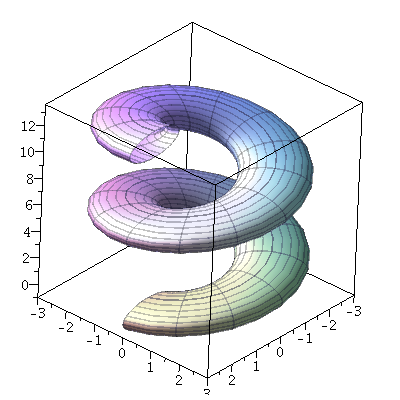
\includegraphics[width=0.5\textwidth]{snake.png}
\end{center}

On the other hand, any surface that can be expressed as a graph or a level surface can also be expressed as a parametric surface. Given a graph $z=f(x,y)$ with $(x,y)\in D\subseteq \R^2$, we can simply define
\[
 \r(x,y) = \langle x, y, f(x,y)\rangle, \quad (x,y)\in D.
\]
Determining a parameterization of a level surface can be harder, but it can always be done in theory (at least locally: this is guaranteed by the Implicit Function Theorem). For example, the ellipsoid $\dfrac{x^2}{6^2}+\dfrac{y^2}{3^2}+\dfrac{z^2}{2^2}=1$ can be parameterized by adapting spherical coordinates, as follows (see Figure 2):
\[
 \r(u,v) = \langle 6\sin u\cos v, 3\sin u\sin v, 2\cos u\rangle, \quad u\in [0,\pi], \, \, v\in [0,2\pi].
\]
\textbf{Exercise:} Verify that this parameterization satisfies the equation of the ellipsoid. That is, show that $\dfrac{x(u,v)^2}{6^2}+\dfrac{y(u,v)^2}{3^2}+\dfrac{z(u,v)^2}{2^2}=1$.

\begin{figure}
\begin{center}
 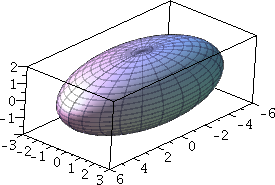
\includegraphics[width=0.6\textwidth]{ellipsoid.png}
\end{center}
\caption{The ellipsoid $\r(u,v) = \langle 6\sin u\cos v, 3\sin u\sin v, 2\cos u\rangle$. The grid lines shown correspond to the curves $u=$constant and $v=$constant.}
\end{figure}

\subsubsection{Exercises 1: Parameterizing surfaces}
\begin{enumerate}
 \item Each of the vector-valued functions below describes a surface you're already familiar with. Identify the surface.
\begin{enumerate}
 \item $\di \r(u,v) = (u+v)\i+(3-v)\j+(1+4u+5v)\k = \begin{bmatrix}0\\3\\1\end{bmatrix}+u\begin{bmatrix}1\\0\\5\end{bmatrix}+v\begin{bmatrix}1\\-1\\5\end{bmatrix}$
 \item $\di \r(u,v) = \langle 2\sin u, 3\cos u, v\rangle$, $u\in [0,2\pi]$, $v\in [0,3]$
 \item $\di \r(u,v) = \langle s, t, t^2-s^2\rangle$, $(s,t)\in \R^2$.
\end{enumerate}
 \item Find a parameterization of the given surface:
\begin{enumerate}
 \item The plane that passes through the point $(1,2,3)$ and is parallel to the vectors $\langle 2,-1,3\rangle$ and $\langle -3, 2, -4\rangle$.
 \item The plane $2x-3y+6z=5$. (Hint: treat the equation of the plane as a system of one linear equation in three variables. The general solution will have two parameters.)
 \item The parboloid $z=4x^2+9y^2$.
 \item The portion of the sphere $x^2+y^2+z^2=9$ with $x,y,z\geq 0$.
 \item The part of the hyperboloid $x^2+y^2-z^2=1$ corresponding to $y\geq 0$. (This one is more challenging; you're probably going to need hyperbolic functions.)
\end{enumerate}

\end{enumerate}
 \subsection{Tangent planes}
Define a parametric surface $S$ by a map $\Phi:D\subseteq \R^2\to \R^3$, given by $\Phi(u,v) = (x(u,v), y(u,v), z(u,v))$ . The derivative of this map is $D_{(u,v)}\Phi = \begin{bmatrix} x_u & x_v\\y_u&y_v\\z_u&z_v\end{bmatrix} = [\Phi_u | \Phi_v]$, where 
\begin{align*}
 \Phi_u(u,v) &= \langle x_u(u,v), y_u(u,v), z_u(u,v)\rangle\\
 \Phi_v(u,v) &= \langle x_v(u,v), y_v(u,v), z_v(u,v)\rangle\\
\end{align*}
are the partial derivatives of $\Phi$ with respect to $u$ and $v$, viewed as vectors. Notice that holding either $u$ or $v$ constant produces a curve that lies on the surface. We obtain the curves
\begin{align*}
 \r_1(u) &= \langle x(u,v_0), y(u,v_0), z(u,v_0)\rangle \quad \text{ (setting $v=v_0$ constant)}\\
 \r_2(v) &= \langle x(u_0,v), y(u_0,v), z(u_0, v)\rangle \quad \text{ (setting $u=u_0$ constant),}
\end{align*}
and at  the point $(u_0,v_0)$, we have the tangent vectors $\r_1'(u_0) = \Phi_u(u_0,v_0)$ and $\r_2'(v_0)=\Phi_v(u_0,v_0)$, which are both tangent to $S$ at the point $(u_0,v_0)$. Since both vectors are tangent to the surface at $(u_0,v_0)$, it follows that their cross product (assuming this is non-zero) is normal to the surface at $(u_0,v_0)$. We obtain the following:
\begin{theorem}
 Let $S\subseteq \R^3$ be a surface parameterized by $\r(u,v) = \langle x(u,v), y(u,v), z(u,v)\rangle$, $(u,v)\in D\subseteq \R^2$. Then a normal vector to the surface at the point $\r(u_0,v_0)$, for $(u_0,v_0)$ in $D$ is given by
\[
 \N(u_0,v_0) = \r_u(u_0,v_0)\times \r_v(u_0,v_0).
\]
\end{theorem}

\begin{figure}[h]
 \begin{center}
  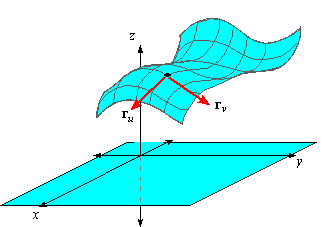
\includegraphics[width=0.3\textwidth]{tangent1.png} \hspace{24pt} 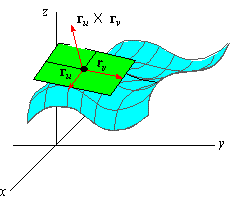
\includegraphics[width=0.3\textwidth]{tangent2.png}
 \end{center}
\caption{The tangent vectors $\r_u$ and $\r_v$, and the tangent plane that contains them.}
\end{figure}

\begin{definition}
 We say that a parametric surface $S$ is \textbf{smooth} if it can be described by a parameterization $\r(u,v) = \langle x(u,v), y(u,v), z(u,v)\rangle$, $(u,v)\in D\subseteq\R^2$ where $\r$ is a $C^1$ vector-valued function of $u$ and $v$, and if $\N(u,v) = \r_u(u,v)\times \r_v(u,v) \neq \mathbf{0}$ for all $(u,v)\in D$.
\end{definition}
Thus, a parametric surface is smooth if it has a well-defined normal vector at each point. Of course, if we have a normal vector at every point, then we should also expect a tangent plane at every point, which agrees with our previous definition of smoothness for a surface. Rather than trying to give a general equation for the tangent plane (which would be rather complicated), we simply note that we've already provided all the ingredients: to define a plane we need a point on the plane, and a normal vector. The point on the plane is of course the point on the surface where we are finding the tangent plane, given by $\r(u_0,v_0)$, and the normal vector is given by $\N(u_0,v_0)$, as above.


\begin{example}
 Find the equation of the tangent plane to the surface $S$ with parametric equations $x=u^2$, $y=u\sin v$, $z=u\cos v$, $u\in [0,\infty)$, $v\in [0,2\pi]$ at the point $(4,0,2)$.

\bigskip

\textbf{Solution:} We identify the surface with the vector-valued function $\r(u,v) = \langle u^2, u\sin v, u\cos v\rangle$. (Notice that $y^2+z^2 = x$, so the surface is in fact a circular paraboloid, but we will not need this fact.) We then have
\begin{align*}
 \r_u(u,v) & = \langle 2u, \sin v, \cos v\rangle\\
 \r_v(u,v) & = \langle 0, u\cos v, -u\sin v\rangle\\
 \N(u,v) & = \r_u(u,v)\times r_v(u,v) \\
& = \begin{vmatrix}
     \i&\j&\k\\2u& \sin v & \cos v\\0 & u\cos v & -u\sin v
    \end{vmatrix}\\
& = -u\i+2u^2\sin v\j + 2u^2\cos v\k.
\end{align*}
Now, we need the normal vector at the given point. We have $x=4=u^2$, so $u=\pm 2$, but we're given $u\geq 0$, so $u=2$. Now we note that $z=2=2\cos v$, which gives $\cos v=1$, so $v=0$, and we can check that this works for $y=0$ as well. (We could take $v=2\pi$ as well; we generally want $\r$ to be one-to-one, but this usual redundancy with trig functions is one of the places where we can relax this requirement.)

We then have $\N(2,0) = -2\i+8\k$ for the normal vector to the surface at $(4,0,2)$ so the equation of the plane is $-2(x-4)+8(z-2)=0$.
\end{example}

\subsubsection{Exercises 2: Finding tangent planes}
Find the tangent plane to the given parametric surface at the given point:
\begin{enumerate}
 \item $\r(u,v) = \langle 2u, u^2+v, v^2\rangle$, at the point $(0,1,1)$. (You will need to determine $(u_0,v_0)$ from the point $(0,1,1)$.)
 \item $\r(u,v) = \langle u^2-v^2, u+v, u^2+4v\rangle$, for $(u,v)=(0,\frac{1}{2})$.
 \item $\r(u,v) = \langle uv, u\sin v, v\cos u\rangle$, for $(u,v) = (0,\pi)$.
\end{enumerate}

\subsection{Surface area}
Recall that for a parametric curve $C$ given by $\r(t)$, $t\in [a,b]$, we have the arc length element $ds = \len{\r'(t)}\,dt$, which describes how much each infinitesimal element of the interval $[a,b]$ is stretched (or shrunk) to produce the curve, and the length of the curve is given by
\[
 s = \int_C\,ds = \int_a^b\len{\r'(t)}\,dt.
\]
Similarly, for a parametric surface $S$ given by $\r(u,v)$, $(u,v)\in D$, we need to know how much the area element $du\,dv$ in $D$ is strectched at each point to produce the surface. The argument is very similar to the one used to justify the change of variables formula. We imagine a little rectangle in the $(u,v)$-plane with bottom-left corner at $(u_0,v_0)$, and sides spanned by the vectors $\Delta u\i$ and $\Delta v\j$. Now we notice that
\begin{align*}
 D_{(u_0,v_0)}\r(\Delta u\i) &= \begin{bmatrix} x_u & x_v\\y_u&y_v\\z_u&z_v\end{bmatrix}\begin{bmatrix}\Delta u\\0\end{bmatrix} = \Delta u\begin{bmatrix}x_u\\y_u\\z_u\end{bmatrix} = \Delta u\r_u(u_0,v_0)\\
 D_{(u_0,v_0)}\r(\Delta v\j) &= \begin{bmatrix} x_u & x_v\\y_u&y_v\\z_u&z_v\end{bmatrix}\begin{bmatrix}0\\ \Delta v\end{bmatrix} = \Delta v\begin{bmatrix}x_v\\y_v\\z_v\end{bmatrix} = \Delta v\r_v(u_0,v_0),
\end{align*}
so the derivative matrix maps the two sides of our rectangle to two vectors tangent to the surface at the point $\r(u_0,v_0)$, and these two vectors span a parallelogram whose area is given by
\[
 \Delta S = \len{(\Delta u\r_u(u_0,v_u))\times (\Delta v\r_v(u_0,v_0))} = \len{\N(u_0,v_0)}\Delta u\Delta v.
\]
From this, we can conclude that the appropriate scale factor is given by the length of the normal vector, just as the scale factor for curves is given by the length of the tangent vector. From this result we obtain the following;
\begin{theorem}
 Let $S$ be a surface given by a smooth, one-to-one\footnote{Requiring $\r(u,v)$ to be one-to-one is a little bit restrictive. In general we can allow the surface to intersect itself; we just want to rule out the possibility that $\r(u,v)$ traces out some portion of the surface more than once, duplicating the area of that portion.} parameterization $\r(u,v)$, $(u,v)\in D$, where $D\subseteq\R^2$ is closed and bounded. (We don't want $D$ to go off to infinity or the area could be infinite.) Then the area of $S$ is given by
\[
 A(S) = \iint_S \,dS = \iint_D\len{\N(u,v)}\,du\,dv.
\]
\end{theorem}
\begin{example}
 Find the area of the surface $S$ parameterized by $\r(u,v) = \langle u-v, u+v, uv\rangle$, with $u^2+v^2\leq 1$.

\textbf{Solution:} We first calculate the normal vector
\[
 \N(u,v) = \langle 1,1,v\rangle\times\langle-1, 1,u\rangle = \langle u-v, -u-v, 2\rangle,
\]
whose length is given by
\[
 \len{\N(u,v)} = \sqrt{(u-v)^2+(-(u+v))^2+2^2} = \sqrt{2u^2+2v^2+4},
\]
so the surface area is given by 
\[
 A(S) = \iint_D \len{\N(u,v)}\,du\,dv = \iint_D \sqrt{2u^2+2v^2+4}\,du\,dv = \int_0^{2\pi}\int_0^1 \sqrt{2r^2+4}r\,dr\,d\theta = \frac{\pi}{3}(6^{3/2}-8).
\]
\end{example}

\subsubsection{Exercises 3: surface area}
Find the area of the following surfaces:
\begin{enumerate}
 \item The part of the plane $2x+5y+z=10$ that lies inside the cylinder $x^2+y^2=9$.
 \item The part of the surface $z=1+3x+2y^2$ that lies above the triangle with vertices $(0,0), (0,1), (2,1)$
 \item The surface $z=x^{3/2}+y^{3/2}$, for $0\leq x\leq 1$, $0\leq y\leq x$
\end{enumerate}

\section{Surface integrals}
As with line integrals, we can define integrals of both scalar and vector fields over a surface. Given a function $f(x,y,z)$ defined and continuous on a surface $S$ with parameterization $\r(u,v)$, $(u,v)\in D$, we can define the integral of $f$ over $S$ by
\[
 \iint_S f(x,y,z)\,dS = \iint_D f(\r(u,v))\len{\N(u,v)}\,du\,dv.
\]
Interpretations of such integrals are similar to those of line integrals of scalar vector fields, and the same sort of computational difficulties arise. Because of this, we tend to focus more on surface integrals of vector fields, just as was the case for line integrals.

The surface integral of a vector field is closely related to the physical concept of \textbf{flux}: if our vector field is interpreted physically as a representing a fluid flow, or an electric field, or some other phenomenon, we are often interested in the total rate of flow over a surface. This is the notion of flux.

One problem arises if we want to talk about flow across a surface: we need to be able to tell one side of the surface from the other, \textbf{for the entire surface}. For example, if our surface is a sphere, we need to distinguish between the inside of the sphere, and the outside of the sphere. This is usually done by making a choice of normal vector: either ``outward-pointing'', or ``inward-pointing''. If it is possible to make this choice consistently over the entire surface, with $\N\neq \mathbf{0}$ throughout, we say that the surface is \textbf{orientable}. All of the surfaces we will deal with are orientable surfaces, but there are many examples of non-orientable surfaces. The most famous of these is the \textit{M\"obius strip}, which you can form for yourself by taking a strip of paper, twisting one end by 180$^\circ$, and joining the ends together. (There are also lots of good YouTube videos on the subject.) The M\"obius strip has the remarkable property of only having one side.

Given a vector field $\F = \langle P,Q,R\rangle$ in $\R^3$, we wish to compute the flux of $\F$ across an oriented surface $S$. If we think in terms of fluid flow, we can see that the total flow across the surface depends on three things: the rate of flow (magnitude of the vector field), the area of the surface, and the angle at which the flow meets the surface.
\begin{figure}[h]
 \begin{center}
  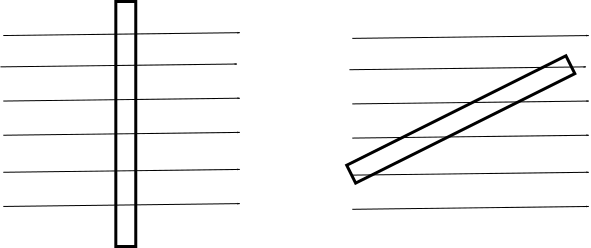
\includegraphics[width=0.5\textwidth]{flux}
 \end{center}
\caption{The flux depends on the magnitude of the vector field (represented by density of arrows), the area of the surface, and the angle between the two. Here we see the effect of angle: fewer arrows cross the second surface, which is of the same area.}
\end{figure}
Putting these together, a reasonable measure of the flux over a portion of the surface is
\[
 \len{\F}\cos\theta \Delta S = (\F\dotp \mathbf{n}) \Delta S,
\]
where $\mathbf{n} = \dfrac{\N}{\len{N}}$ is the unit normal vector. (The normal vector allows us to measure the angle between the vector field and the surface, but since the magnitude of the normal vector depends on the choice of parameterization, we use the unit normal vector to get the flux per unit area.)

The total flux over the surface $S$ is then given by
\[
 \iint_S (\F\dotp\mathbf{n}) dS.
\]
Recall that for the line integral of a vector field over a curve, we have the equivalent integrals
\[
 \int_C (\F\dotp \mathbf{T})\,ds = \int_C \F\dotp \,d\r,
\]
since for any parameterization $\r(t)$ for $C$, we have the arc length element $ds = \len{\r'(t)}\,dt$, the unit tangent vector $\mathbf{T}=\dfrac{\r'(t)}{\len{\r'(t)}}$, and the vector-valued line element $d\r = \r'(t)\,dt$. (We can think of $d\r$ as the vector-valued differential $d\r = \langle dx, dy, dz\rangle$, so that $\F\dotp d\r = P\,dx+Q\,dy+R\,dz$.)

Similarly, for surface integrals, we can define the vector-valued surface element $d\S$, given in terms of a parameterization by $d\S = \N(u,v)\,du\,dv$. For a choice of parameterization $\r(u,v)$, $(u,v)\in D$, this gives us the surface integral
\[
 \iint_S \F\dotp d\S = \iint_D \F(\r(u,v))\dotp\N(u,v)\,du\,dv = \iint_D (\F(\r(u,v))\dotp \mathbf{n}(u,v))\len{\N(u,v)}\,du\,dv = \iint_S (\F\dotp \mathbf{n})\,dS.
\]
Again, you will sometimes see $d\S$ viewed as a vector-valued area element $d\S = \langle dy\,dz, dz\,dx, dx\,dy\rangle$, so that 
\[
 \F\dotp d\S = P(x,y,z)\,dy\,dz+Q(x,y,z)\,dz\,dx+R(x,y,z)\,dx\,dy
\]
\begin{example}
 Evaluate the surface integral $\iint_S\F\dotp d\S$, where $\F(x,y,z) = \langle xy,yz,zx\rangle$, and $S$ is the portion of the paraboloid $z=4-x^2-y^2$ that lies above the square $[0,1]\times [0,1]$, with upward-pointing normal vector.

\bigskip

\textbf{Solution:} Since $S$ is a graph, we use $x$ and $y$ as parameters, so $\r(x,y) = \langle x, y, 4-x^2-y^2\rangle$, with $0\leq x,y\leq 1$. We have
\begin{align*}
 \r_x(x,y) &= \langle 1, 0, -2x\rangle\\
 \r_y(x,y) &= \langle 0, 1, -2y\rangle\\
 \N(x,y) & = \r_x(x,y)\times \r_y(x,y) = \langle 2x, 2y, 1\rangle,
\end{align*}
and since the $z$ component of $\N$ is always positive, we know we have the upward-pointing normal vector. (If we had chosen a parameterization where the $z$ component was negative, we can simply replace $\N$ by $-\N$: changing the orientation reverses the sign of the integral.)

We then have 
\[
\F(x,y,4-x^2-y^2)\dotp \N(x,y) = \langle xy, 4y-x^2y-y^3, 4x-x^3-x^2y\rangle\dotp \langle 2x, 2y, 1\rangle.
\]
Finally, the integral is given by
\[
 \iint_S \F\dotp \,d\S = \int_0^1\int_0^1 (2x^2y+8y^2-2x^2y^2-2y^4+4x-x^3-xy^2)\,dx\,dy = \dfrac{713}{180}.
\]
(Okay, the numbers got ugly, but the procedure was straightforward.)
\end{example}

\subsubsection{Exercises 4: surface integrals}
Evaluate the integral of the given vector field over the given surface.
\begin{enumerate}
 \item $\F(x,y,z) = \langle y, x, z^2\rangle$, $\r(u,v) = \langle u\cos v, u\sin v, v\rangle$, for $u\in [0,1], v\in [0,\pi]$.
 \item $\F(x,y,z) = xze^y\i-xye^y\j +z\k$, where $S$ is the part of the plane $x+y+z=1$ in the first octant (with $x,y,z\geq 0$), with downward-pointing orientation.
 \item $\F(x,y,z) = \langle x, y, z^4\rangle$, $S$ is the part of the cone $z=\sqrt{x^2+y^2}$ that lies beneath the plane $z=1$, with downward-pointing orientation.
 \item $\F(x,y,z) = \langle xz, x, y\rangle$, $S$ is the hemisphere $x^2+y^2+z^2=25$ with $y\geq 0$, oriented in the direction of the positive $y$-axis.
\end{enumerate}
\section{Solutions to Exercises}
\subsection{Exercises 1: Parameterizing surfaces}
\begin{enumerate}
 \item Each of the vector-valued functions below describes a surface you're already familiar with. Identify the surface.
\begin{enumerate}
 \item $\di \r(u,v) = (u+v)\i+(3-v)\j+(1+4u+5v)\k = \begin{bmatrix}0\\3\\1\end{bmatrix}+u\begin{bmatrix}1\\0\\5\end{bmatrix}+v\begin{bmatrix}1\\-1\\5\end{bmatrix}$
 
 \bigskip
 
 We have 
 \[
 \langle x, y, z\rangle = \langle 0, 3, 1\rangle + u\langle 1, 0, 4\rangle + v\langle 1, -1, 5\rangle,
 \]
 so this is a plane through the point $(0,3,1)$ that contains the vectors $\langle 1, 0, 4\rangle$ and $\langle 1, -1, 5\rangle$. Computing the normal vector
 \[
 \N = \langle 1, 0, 4\rangle\times\langle 1, -1, 5\rangle = \langle 4, -1, -1\rangle,
 \]
 we have the scalar equation $4x-(y-3)-(z-1)=0$ for the plane.
 
 \item $\di \r(u,v) = \langle 2\sin u, 3\cos u, v\rangle$, $u\in [0,2\pi]$, $v\in [0,3]$

\bigskip

We have $x=2\sin u$ and $y=3\cos u$, so $\dfrac{x^2}{4}+\dfrac{y^2}{9} = 1$, with $z=v$ a free parameter. This is an elliptical cylinder parallel to the $z$-axis.

 \item $\di \r(u,v) = \langle s, t, t^2-s^2\rangle$, $(s,t)\in \R^2$.

\bigskip

With $x=s$ and $y=t$, we have $z=y^2-x^2$, which is the equation of a hyperbolic paraboloid.

\end{enumerate}
 \item Find a parameterization of the given surface:
\begin{enumerate}
 \item The plane that passes through the point $(1,2,3)$ and is parallel to the vectors $\langle 2,-1,3\rangle$ and $\langle -3, 2, -4\rangle$.

\bigskip

From the given information we have 
\[
\bbm x\\y\\z\ebm = \bbm 1\\2\\3\ebm + s\bbm 2\\-1\\3\ebm + t\bbm -3\\2\\-4\ebm,
\]
so we can take
\[
\r(s,t) = \langle 1+2s-3t, 2-s+2t, 3+3s-4t\rangle.
\]

 \item The plane $2x-3y+6z=5$. (Hint: treat the equation of the plane as a system of one linear equation in three variables. The general solution will have two parameters.)

\bigskip

Solving for $x$, we have $x = 5+\dfrac{3}{2}y-3z$. Setting $y=u$ and $z=v$, we get
\[
\r(u,v) = \langle 5+\frac{3}{2}u-3v, u, v\rangle.
\]
We could also solve for either $y$ or $z$; note that we have
\[
\bbm x\\y\\z\ebm = \bbm 5\\0\\0\ebm + s\bbm 3/2\\1\\0\ebm + t\bbm -3\\0\\1\ebm,
\]
so if desired we can obtain two vectors tangent to the plane, as in the previous problem.

 \item The parboloid $z=4x^2+9y^2$.

\bigskip

Since the surface is given to us as a graph, we can simply take
\[
\r(x,y) = \langle x, y, 4x^2+9y^2\rangle.
\]

 \item The portion of the sphere $x^2+y^2+z^2=9$ with $x,y,z\geq 0$.

\bigskip

Since all three variables are restricted to non-negative values, we can solve for any one of them in terms of the other two. Since we're used to solving for $z$, we take $z=\sqrt{9-x^2-y^2}$, giving us the parameterization
\[
\r(x,y) = \langle x, y, \sqrt{9-x^2-y^2}\rangle,
\]
where $0\leq x\leq 3$ and $0\leq y\leq \sqrt{9-x^2}$. (The parameters $x$ and $y$ belong to the portion of the disk $x^2+y^2\leq 9$ that lies in the first quadrant.)

We can alternatively choose to use polar coordinates as parameters, giving us
\[
\r(r,\theta) = \langle r\cos\theta, r\sin\theta, \sqrt{9-r^2}\rangle,
\]
with $0\leq r\leq 3$ and $0\leq \theta \leq \pi/2$ (since we're in the first octant). Another option is to use spherical coordinates (with $\rho = 3$ constant). This gives us
\[
\r(\phi,\theta) = \langle 3\sin\phi\cos\theta, 3\sin\phi\sin\theta, 3\cos\phi\rangle,
\]
with $0\leq \phi\leq \pi/2$ and $0\leq \theta\leq \pi/2$.


 \item The part of the hyperboloid $x^2+y^2-z^2=1$ corresponding to $y\geq 0$. (This one is more challenging; you're probably going to need hyperbolic functions.)
 
 \bigskip
 
 Note that when $z=0$ we have $x^2+y^2=1$, and $y\geq 0$. This suggests that we can take $x=f(v)\cos u$, $y=g(v)\sin u$, with $u\in [0,\pi]$ (to make sure $y\geq 0$), where $f(u)$ and $g(u)$ are needed to account for the $z$ coordinate. When $y=0$ we have $x^2-z^2=1$, giving us a hyperbola, which can be parameterized using $x=\cosh v$ and $z=\sinh v$ for one half, and $x=-\cosh t$, $z=\sinh t$ for the other half. This suggests that we might be able to take $f(v) = \cosh t v$ for $x$, and a similar argument tells us that the same will work for $y$. 
 
 A bit of thought also tells us that we don't have to worry about the other branch of the hyperbola, where $x<0$, since $\cos\theta\leq 0$ for $\theta \in [\pi/2, .pi]$. Putting everything together, we have
 \[
 \r(u,v) = \langle \cos u\cosh v, \sin u\cosh v, \sinh v\rangle,
 \]
 for $u\in [0,\pi]$ and $v\in\R$. To check that this works, note that
 \[
 x^2+y^2 = \cos^2u\cosh^v+\sin^2u\cosh^2v = \cosh^2v = 1-\sinh^2 v = 1-z^2.
 \]

\end{enumerate}
\end{enumerate}

\subsection{Exercises 2: Finding tangent planes}
Find the tangent plane to the given parametric surface at the given point:
\begin{enumerate}
 \item $\r(u,v) = \langle 2u, u^2+v, v^2\rangle$, at the point $(0,1,1)$. (You will need to determine $(u_0,v_0)$ from the point $(0,1,1)$.)

\bigskip

First, we note that $2u=0$ implies $u=0$, and then $u^2+v=1$ tells us that $v=1$. (We should also confirm that $1^1=1$, so the $z$-coordinate works as well.)

Next, we compute tangent vectors at the given point:
\begin{align*}
 \r_u(u,v) & = \langle 2, 2u, 0\rangle & \text{ so } & \r_u(0,1) = \langle 2, 0, 0\rangle.\\
 \r_v(u,v) & = \langle 0,1,2v\rangle & \text { so } & \r_v(0,1) = \langle 0,1,2\rangle.
\end{align*}
This gives us the normal vector $\N(0,1) = \r_u(0,1)\times \r_v(0,1) = \langle 0,-4,2\rangle$, so the equation of the plane is
\[
 -4(y-1)+2(z-1)=0.
\]


 \item $\r(u,v) = \langle u^2-v^2, u+v, u^2+4v\rangle$, for $(u,v)=(0,\frac{1}{2})$.

\bigskip

We have
\begin{align*}
 \r_u(u,v) & = \langle 2u,1,2u\rangle, \quad \r_u(0, 1/2) = \langle 0, 1, 0\rangle,\\
 \r_v(u,v) & = \langle -2v, 1, 4\rangle, \quad \r_v(0,1/2) = \langle -1, 1, 4\rangle,
\end{align*}
so $\N(0,1/2) = \r_u(0,1/2)\times\r_v(0,1/2) = \langle 4, 0, 1\rangle$. Since $\r(0,1/2) = \langle -1/4, 1/2, 2\rangle$, the equation of the plane is
\[
 4(x+1/4)+z-2 = 0.
\]


 \item $\r(u,v) = \langle uv, u\sin v, v\cos u\rangle$, for $(u,v) = (0,\pi)$.

\bigskip

We have $\r(0,\pi) = \langle 0, 0, \pi\rangle$, and
\begin{align*}
 \r_u(u,v) & = \langle v, \sin v, -v\sin u\rangle, \quad \r_u(0,\pi) = \langle \pi, 0, 0\rangle;
 \r_v(u,v) & = \langle u, u\cos v, \cos u\rangle, \quad \r_v(0,\pi) = \langle 0, 0, 1\rangle,
\end{align*}
so $\N(0,\pi) = (\pi \i)\times \k = -\pi \j$, giving us $y=0$ as the equation of the plane.

\end{enumerate}

\subsection{Exercises 3: surface area}
Find the area of the following surfaces:
\begin{enumerate}
 \item The part of the plane $2x+5y+z=10$ that lies inside the cylinder $x^2+y^2=9$.

\bigskip

Solving for $z$, we have the graph $z=10-2x-5y$, so $\r(x,y) = \langle x, y, 10-2x-5y\rangle$, which gives us (exercise) $\N(x,y) = \langle 2, 5, 1\rangle$, so $\len{\N(x,y)} = \sqrt{30}$. The parameter domain $D$ is given by the disc $x^2+y^2\leq 9$, so we have
\[
 A(S) = \iint_S \,dS = \iint_D \len{N(x,y)}\,dA = \iint_D\sqrt{30}\,dA = \sqrt{30}(9\pi),
\]
since the area of the disc $D$ is $\pi(3^2)=9\pi$.

 \item The part of the surface $z=1+3x+2y^2$ that lies above the triangle with vertices $(0,0), (0,1), (2,1)$

\bigskip

We parameterize our graph using $\r(x,y) = \langle x, y, 1+3x+2y^2\rangle$, giving us
\begin{align*}
 \r_x(x,y) & = \langle 1, 0, 3\rangle\\
 \r_y(x,y) & = \langle 0, 1, 4y\rangle\\
 \N(x,y) & = \langle -3, -4y, 1\rangle\\
 \len{\N(x,y)} & = \sqrt{10+16y^2}.
\end{align*}
Our parameter domain $D$ can be described as the Type 2 region $0\leq y\leq 1$, $0\leq x\leq 2y$, so we have
\[
 A = \iint_D\len{\N(x,y)}\,dA = \int_0^1\int_0^{2y}\sqrt{10+16y^2}\,dx\,dy = \int_0^1 2y\sqrt{10+16y^2}\,dy = \frac{1}{24}(26^{3/2}-10^{3/2}).
\]

 \item The surface $z=x^{3/2}+y^{3/2}$, for $0\leq x\leq 1$, $0\leq y\leq x$

\bigskip

Again we have a graph, so we take $\r(x,y) = \langle x, y, x^{3/2}+y^{3/2}\rangle$. This gives us
\begin{align*}
 \r_x(x,y) & = \langle 1, 0, \frac{3}{2}\sqrt{x}\rangle\\
 \r_y(x,y) & = \langle 0, 1, \frac{3}{2}\sqrt{y}\rangle\\
 \N(x,y) & = \langle -\frac{3}{2}\sqrt{x}, -\frac{3}{2}\sqrt{y}, 1\rangle\\
 \len{\N(x,y)} & = \sqrt{\frac{9}{4}(x+y)+1}
\end{align*}
The area integral can be done by hand, but it's... ugly. 

\end{enumerate}
\subsection{Exercises 4: surface integrals}
Evaluate the integral of the given vector field over the given surface.
\begin{enumerate}
 \item $\F(x,y,z) = \langle y, x, z^2\rangle$, $\r(u,v) = \langle u\cos v, u\sin v, v\rangle$, for $u\in [0,1], v\in [0,\pi]$.

\bigskip

We have $\F(\r(u,v)) = \langle u\sin v, u\cos v, v^2\rangle$, and the normal vector is $\N(u,v) = \langle \sin v, -\cos v, u\rangle$, so we have
\begin{align*}
 \iint_S\F\dotp\,d\S & = \int_0^{\pi}\int_0^1 \F(\r(u,v))\dotp\N(u,v)\,du\,dv\\
& = \int_0^\pi\int_0^1 (u\sin^2v-u\cos^v+uv^2)\,du\,dv\\
& = \int_0^{\pi}(\frac{1}{2}v^2-\frac{1}{2}\cos(2v))\,dv = \frac{\pi^3}{6}.
\end{align*}

 \item $\F(x,y,z) = xze^y\i-xye^y\j +z\k$, where $S$ is the part of the plane $x+y+z=1$ in the first octant (with $x,y,z\geq 0$), with downward-pointing orientation.

\bigskip

We can parameterize the plane by solving for $z=1-x-y$, so $\r(x,y) = \langle x, y, 1-x-y\rangle$, where $(x,y)\in D$, and $D$ is the region in the $xy$-plane bounded by the coordinate axes and the line $x+y=1$ (so either $0\leq y\leq x$ where $0\leq x\leq 1$, or $0\leq x\leq y$ where $0\leq y\leq 1$). This parameterization gives us the normal vector $\N(x,y) = \langle 1, 1, 1\rangle$, which is upward-pointing, so we will have to remember to change our sign to account for orientation.

This gives us
\begin{align*}
 \iint_S\F\dotp\,d\S & = -\iint_D\langle x(1-x-y)e^y, -xye^y, 1-x-y\rangle\dotp \langle 1, 1, 1\rangle\,dA\\
 & = -\int_0^1\int_0^x(xe^y-x^2e^y-2xye^y+1-x-y)\,dy\,dx,
\end{align*}
which results in a big mess, but it can be done in principle. (I mis-typed the problem: the $y$-component should have been $-xze^y$, and then things simplify nicely. Instead you get a whole lot of integration by parts.)




 \item $\F(x,y,z) = \langle x, y, z^4\rangle$, $S$ is the part of the cone $z=\sqrt{x^2+y^2}$ that lies beneath the plane $z=1$, with downward-pointing orientation.

\bigskip

Our surface is a graph, so we take $\r(x,y) = \langle x, y, \sqrt{x^2+y^2}\rangle$, with $x^2+y^2\leq 1$. (The parameter domain is determined by the requirement that $0\leq z\leq 1$.) The normal vector for this parameterization is $\N(x,y) = \left\langle -\dfrac{x}{\sqrt{x^2+y^2}}, -\dfrac{y}{\sqrt{x^2+y^2}}, 1\right\rangle$, which is opposite to the assigned orientation, so we will need to change the sign. With $z=\sqrt{x^2+y^2}$, our vector field is
\[
 \F(x,y,\sqrt{x^2+y^2}) = \langle x, y, (x^2+y^2)^2\rangle,
\]
so
\begin{align*}
 \iint_S\F\dotp\,d\S & = -\iint_D \langle x, y, (x^2+y^2)^2\rangle\dotp \left\langle -\frac{x}{\sqrt{x^2+y^2}}, -\frac{y}{\sqrt{x^2+y^2}}, 1\right\rangle\,dA\\
& = -\iint_D \left(\frac{-x^2-y^2}{\sqrt{x^2+y^2}}+(x^2+y^2)^2\right)\,dA\\
& = -\int_0^{2\pi}\int_0^1 (-r+r^4)r\,dr\,d\theta\\
& = -2\pi\left(-\frac{1}{3}+\frac{1}{6}\right) = \frac{\pi}{3}.
\end{align*}



 \item $\F(x,y,z) = \langle xz, x, y\rangle$, $S$ is the hemisphere $x^2+y^2+z^2=25$ with $y\geq 0$, oriented in the direction of the positive $y$-axis.

\bigskip

We went over this one in class: doing it directly is a mess, whatever parameterization you choose, and the whole thing ends up simplifying to zero if you're able to push through it. A cleaner solution involves using the divergence theorem to relate the integral over $S$ to the integral over the disc $x^2+z^2=25$ in the $xz$-plane.
\end{enumerate}

\end{document}